\documentclass[11pt]{article}

\usepackage[utf8]{inputenc}
\usepackage[T1]{fontenc}
\usepackage{lmodern}
\usepackage[a4paper,margin=0.88in]{geometry}
\usepackage{amsmath,amssymb,amsthm,mathtools}
\usepackage{xcolor}
\usepackage[most]{tcolorbox}
\usepackage{booktabs,array,tabularx}
\usepackage{enumitem}
\usepackage{titlesec}
\usepackage{parskip}
\usepackage{tikz}
\usetikzlibrary{arrows.meta,positioning,fit,calc}
\usepackage[colorlinks=true,linkcolor=blue!55!black,urlcolor=blue!60!black,citecolor=blue!55!black]{hyperref}

\definecolor{accent}{HTML}{45358F}
\definecolor{accent2}{HTML}{087E8B}
\definecolor{accent3}{HTML}{B45309}
\definecolor{soft}{HTML}{F4F2FB}
\definecolor{cool}{HTML}{E8F6F7}
\definecolor{warm}{HTML}{FFF4E6}
\definecolor{risk}{HTML}{A61B1B}

\titleformat{\section}{\Large\bfseries\color{accent}}{\thesection}{0.55em}{}
\titleformat{\subsection}{\large\bfseries\color{accent!85!black}}{\thesubsection}{0.55em}{}
\titlespacing*{\section}{0pt}{1.4em}{0.5em}

\newtcolorbox{keybox}[1][]{colback=soft,colframe=accent,boxrule=.7pt,arc=2pt,
  left=7pt,right=7pt,top=5pt,bottom=5pt,fonttitle=\bfseries,#1}
\newtcolorbox{theorybox}[1][]{colback=cool,colframe=accent2,boxrule=.7pt,arc=2pt,
  left=7pt,right=7pt,top=5pt,bottom=5pt,fonttitle=\bfseries,title={Theory target},#1}
\newtcolorbox{riskbox}[1][]{colback=red!3,colframe=risk,boxrule=.7pt,arc=2pt,
  left=7pt,right=7pt,top=5pt,bottom=5pt,fonttitle=\bfseries,title={Falsification gate},#1}
\newtcolorbox{claimbox}[1][]{colback=warm,colframe=accent3,boxrule=.8pt,arc=2pt,
  left=7pt,right=7pt,top=5pt,bottom=5pt,fonttitle=\bfseries,title={Claim allowed only if the experiments support it},#1}

\newtheorem{proposition}{Proposition}
\newtheorem{targettheorem}{Target theorem}
\newtheorem{lemma}{Lemma}

\newcommand{\R}{\mathbb{R}}
\newcommand{\E}{\mathbb{E}}
\newcommand{\norm}[1]{\left\lVert #1\right\rVert}
\newcommand{\softmax}{\operatorname{softmax}}
\newcommand{\Attn}{\operatorname{Attn}}
\newcommand{\bytes}{\operatorname{Bytes}}
\newcommand{\cost}{\operatorname{Cost}}
\newcommand{\term}[1]{\textbf{\color{accent!85!black}#1}}

\begin{document}
\pagenumbering{roman}

\begin{titlepage}
\centering
\vspace*{1.25cm}
{\Huge\bfseries\color{accent} CATT-KV\par}
\vspace{0.25cm}
{\Large\bfseries Causal Attention-Aware Tensor-Train\ KV-Cache Compression\par}
\vspace{0.45cm}
{\large SVD-free block updates, RoPE-equivariant tensor contraction,\ sparse innovations, and reconstruction-free attention\par}
\vspace{1.0cm}
\begin{tcolorbox}[colback=soft,colframe=accent,width=.94\textwidth,arc=3pt]
\centering\bfseries
CATT-KV asks whether an evolving KV cache can be stored as causally appendable tensor cores and
consumed directly by attention, so that compression reduces both capacity and bytes read per
decoded token rather than creating a decompression bottleneck.
\end{tcolorbox}
\vspace{.7cm}
\begin{tcolorbox}[colback=warm,colframe=accent3,width=.94\textwidth,arc=3pt]
\small
\textbf{Positioning.} This is a \emph{Technique Paper}, not ``Tucker instead of SVD.'' Its novelty
must come from the complete mechanism: dyadic causal tensorization, an SVD-free attention-weighted
update, analytic RoPE handling, direct core-domain attention, and a payback rule that declines to
compress when runtime savings cannot recover compression cost.
\end{tcolorbox}
\vfill
{\normalsize Rigorous research proposal \;\textbullet\; July 2026\par}
\end{titlepage}

\tableofcontents
\newpage
\pagenumbering{arabic}

\section{Executive decision}

\begin{keybox}[title={One-sentence key idea}]
Tensorize each aged KV block along causal position digits, represent it with SVD-free
Tensor-Train cores plus attention-critical sparse innovations, and evaluate RoPE attention
directly from those cores without materializing dense keys or values.
\end{keybox}

The project has high upside but a hard empirical gate. Tensor-Train (TT) storage is irrelevant if
enumerating logits or updating cores is slower than reading dense or INT4 KV. Accordingly, the
first deliverable is not a full model integration; it is a payback study on recorded per-layer KV
blocks. Only a positive memory--latency--quality frontier authorizes the full implementation.

\begin{center}
\small
\renewcommand{\arraystretch}{1.22}
\begin{tabularx}{.98\textwidth}{@{}p{2.55cm}X p{2.2cm}@{}}
\toprule
\textbf{Axis} & \textbf{Required contribution} & \textbf{Gate} \\
\midrule
Representation & Causal TT over token digits, with RoPE-pair structure retained & $\ge 4\times$ physical KV reduction before factor quantization \\
Quality & Attention-output objective and structured sparse correction & $<1$ LongBench point or $<2\%$ relative PPL loss \\
Runtime & Fused logits/value contraction, no dense old-KV reconstruction & $\ge1.3\times$ long-context decode speedup \\
Amortization & Compress a block once when it ages; admit only positive-payback blocks & $<5\%$ amortized overhead \\
Baseline strength & Compare at matched physical bytes against low-bit quantization & Beat the INT4 Pareto frontier on at least one system axis \\
\bottomrule
\end{tabularx}
\end{center}

\section{Research gap and novelty boundary}

The KV cache for a decoder layer is naturally a tensor over KV head, token position, and feature.
However, ``using a tensor'' is not new. DecoQuant uses a matrix-product-operator decomposition to
redistribute outliers before quantization~\cite{decoquant}; JoLT compresses token and feature axes
with partial Tucker plus a rotated low-bit residual~\cite{jolt}; Tucker-KV publicly proposed
HOSVD/HOOI refinement and rank allocation~\cite{tuckerkv}. Matrix methods already cover offline
low-rank projection (Palu and Eigen Attention)~\cite{palu,eigen}, online subspace updates
(OjaKV)~\cite{ojakv}, and RoPE-aligned reconstruction avoidance (RAP)~\cite{rap}.

\begin{center}
\scriptsize
\renewcommand{\arraystretch}{1.23}
\begin{tabularx}{\textwidth}{@{}p{2.1cm}p{2.4cm}p{2.25cm}p{2.25cm}X@{}}
\toprule
\textbf{Method family} & \textbf{Representation} & \textbf{Online update} & \textbf{Dense reconstruction} & \textbf{Gap left for CATT-KV} \\
\midrule
Palu / Eigen & Matrix projection & No / calibration & Full or fused projection path & No causal multiway model \\
OjaKV & Adaptive matrix basis & Periodic PCA-style & Reconstructed approximate KV & No tensor cores or direct TT attention \\
DecoQuant & MPO local tensors & Data-free transform & Dequantization path & Tensorization serves quantization, not causal direct attention \\
JoLT & Partial Tucker + residual & Block compression & Representation-focused & Uses HOSVD/randomized-SVD family; no causal TT execution path \\
RAP & RoPE-pair pruning & No & Avoided through aligned absorption & Pruning, not data-adaptive tensor compression \\
\textbf{CATT-KV} & Causal TT + sparse innovation & SVD-free, blockwise & \textbf{Never for old blocks} & Attention-aware, RoPE-equivariant, payback-gated \\
\bottomrule
\end{tabularx}
\end{center}

\begin{claimbox}
The publishable novelty is \emph{not} TT alone. It is an attention-executable, causal TT cache:
the decomposition algorithm, positional operator, error correction, kernel, and admission rule
are designed as one inference mechanism.
\end{claimbox}

\section{Thinking template and logic chain}

\small
\renewcommand{\arraystretch}{1.18}
\begin{tabularx}{\textwidth}{@{}p{3.35cm}X@{}}
\toprule
\textbf{Stage} & \textbf{Proposal content} \\
\midrule
Research background & Long-context decoding repeatedly reads an expanding KV cache. Quantization,
projection, eviction, and recent Tucker methods reduce storage, but runtime wins depend on whether
attention can consume the representation without expensive update or reconstruction. \\
Limitation 1 & Tucker/MPO cache methods do not provide a causally appendable SVD-free TT update
whose cost is explicitly amortized against future KV reads. \\
Limitation 2 & Generic low-rank representations ignore RoPE's position-dependent pair rotations;
naive projection can force reconstruction or inflate rank. \\
Limitation 3 & Frobenius reconstruction loss and byte count do not control softmax routing or
end-to-end latency. \\
Key idea & Store aged causal blocks as RoPE-aware TT cores plus attention-critical sparse
innovations and compute attention directly in that domain. \\
Challenge 1 & A growing sequence changes tensor extent, while per-token decomposition would erase
the expected latency savings. \\
Challenge 2 & Query-dependent softmax and RoPE must be evaluated without expanding a $B\times d$
block. \\
Challenge 3 & Low tensor error can still change attention routing; rank and residual budgets must
optimize quality, bytes, and payback jointly. \\
Module A & Age-triggered SVD-free TT fitting and a block admission controller. \\
Module B & RoPE-equivariant direct TT logits and value aggregation kernels. \\
Module C & Query-sketch-weighted ranks plus structured sparse innovations and error bounds. \\
Contributions & C1 causal TT cache (Sec.~\ref{sec:representation}); C2 direct RoPE tensor attention
(Sec.~\ref{sec:direct}); C3 quality/payback controller and guarantees
(Secs.~\ref{sec:objective}--\ref{sec:theory}); C4 reproducible system evaluation
(Sec.~\ref{sec:experiments}). \\
\bottomrule
\end{tabularx}
\normalsize

All four consistency checks pass: each limitation is answered by the key idea; each challenge is a
mechanism-level consequence of implementing it; Modules A--C map one-to-one to the challenges;
and every contribution names a method or evaluation section. There are no orphan modules.

\section{Formal problem statement}

For layer $\ell$, KV head $h$, and a closed block $b$ of $B$ token positions, let
\[
K_{\ell hb},V_{\ell hb}\in\R^{B\times d}, \qquad
o(q)=\softmax(qK_{\ell hb}^{\top}/\sqrt d)V_{\ell hb}.
\]
The exact recent window remains in the model's native layout. CATT-KV applies only to a block after
it leaves that window. The method must choose a representation $\mathcal C_b$, sparse correction
$E_b$, and execution kernel satisfying a physical memory budget $M$ and an update budget $T_c$:
\begin{align}
\min_{\mathcal C_b,E_b}\quad &
\E_{q\sim\mathcal Q_b}\!\left[\norm{o(q)-\widehat o(q;\mathcal C_b,E_b)}_2^2\right]
+\lambda\bytes(\mathcal C_b,E_b)+\mu\cost_{\rm decode}(\mathcal C_b,E_b), \label{eq:objective}\\
\text{s.t.}\quad &\cost_{\rm compress}(b)\le T_c,
\quad \mathcal C_b\text{ is consumed without dense }K_b,V_b. \nonumber
\end{align}
Here $\mathcal Q_b$ is a causal query sketch from prompt and recent-query statistics. Since future
queries are unknown, the empirical term is paired with a norm-based robust bound in
Section~\ref{sec:theory}.

\section{Causal TT representation}
\label{sec:representation}

Factor $B=\prod_{j=1}^{p}n_j$ (usually $n_j=2$ or $4$) and map token position
$s\leftrightarrow(i_1,\ldots,i_p)$. For one head,
\[
\mathcal K_b[i_1,\ldots,i_p,c]
\approx G_1^K[i_1]G_2^K[i_2]\cdots G_p^K[i_p]G_{p+1}^K[c],
\]
where $G_j[i_j]\in\R^{r_{j-1}\times r_j}$, $r_0=r_{p+1}=1$, and $c\in[d]$.
The value cache has separate cores because K and V have different spectra and roles.

\begin{proposition}[Physical TT storage]
Ignoring alignment and metadata, one K block requires
$\sum_{j=1}^{p}r_{j-1}n_jr_j+r_pd$ scalars, rather than $Bd$. The implementation reports actual
allocated bytes, including rank tables, sparse indices, padding, and quantization scales.
\end{proposition}

Heads are initially decomposed independently to avoid forcing unrelated head bases. A later ablation
adds the head as a TT mode only when it reduces physical bytes without raising contraction cost.
This prevents a common tensor-paper mistake: assuming every available axis should be jointly
factorized.

\subsection{Age-triggered SVD-free update}

Standard TT-SVD is excluded because it repeatedly invokes matrix SVD. CATT-KV instead uses a
warm-started, fixed-sweep TT-ALS update, with QR or regularized least-squares core solves. Online
TT-ALS supplies a relevant streaming foundation~\cite{onlinett}; randomized streaming sketches
offer an alternative when dense MTTKRP-like passes are too expensive~\cite{stta}.

\begin{keybox}[title={Block lifecycle}]
\textbf{Open:} append native K/V to the exact hot block. \quad
\textbf{Close:} freeze the block after $B$ tokens. \quad
\textbf{Fit once:} run at most $J$ TT-ALS sweeps and select sparse innovations. \quad
\textbf{Admit or reject:} retain TT only if predicted payback is positive; otherwise store INT4 or
native KV. \quad
\textbf{Consume:} use direct TT attention for every later query.
\end{keybox}

\section{Attention-aware fitting and sparse innovations}
\label{sec:objective}

Pure TT-ALS minimizes tensor reconstruction. CATT-KV changes the local weighting using a small
query sketch $Q_b=[q_1,\ldots,q_m]$ and a robust residual term. For a candidate approximation,
define token influence
\begin{align}
I^K_s &= \max_{q\in\mathcal Q_b}\frac{|q^\top(K_s-\widehat K_s)|}{\sqrt d}
+\rho\norm{K_s-\widehat K_s}_2,\\
I^V_s &= \bar\alpha_s\norm{V_s-\widehat V_s}_2,
\end{align}
where $\bar\alpha_s$ is a conservative attention-mass estimate. The residual stores the largest
token--RoPE-pair blocks under $I_s^K+I_s^V$, rather than arbitrary scalar entries. This alignment
keeps gather operations coalesced and permits exact pair rotations.

Rank selection minimizes an empirical Lagrangian
\[
\widehat L(\mathbf r,k)=L_{\rm attn}(\mathbf r,k)
+\lambda M(\mathbf r,k)+\mu C_{\rm decode}(\mathbf r,k)+\nu C_{\rm fit}(\mathbf r,k),
\]
where $k$ is the residual-block budget. A greedy controller grows the bond or residual budget with
the largest measured loss reduction per added byte, subject to a payback constraint. No claim of
globally optimal tensor rank allocation is made.

\section{RoPE-equivariant direct TT attention}
\label{sec:direct}

Let $\bar k_s$ be the pre-RoPE key and $R_s$ the block-diagonal RoPE matrix. A query at position
$t$ uses
\[
(R_tq)^\top(R_s\bar k_s)=q^\top R_{s-t}\bar k_s.
\]
For frequency pair $j$, $R_{s-t}$ is a $2\times2$ rotation containing
$\cos((s-t)\theta_j)$ and $\sin((s-t)\theta_j)$. Under a dyadic encoding of $s$, the complex
sequence $e^{\mathrm i s\theta_j}$ factorizes across position bits; its real representation has
TT rank at most two for a fixed frequency. CATT-KV therefore constructs the position operator
analytically and fuses it with the feature-core contraction instead of rotating or reconstructing
all keys.

\begin{lemma}[Fixed-frequency RoPE tensorization]
If $s=\sum_{m=0}^{p-1}2^mi_m$, then
$e^{\mathrm i s\theta}=\prod_m e^{\mathrm i2^mi_m\theta}$. Hence the complex exponential has
rank-one dyadic TT form; the coupled real sine/cosine representation has rank at most two.
\end{lemma}

The key kernel first contracts the feature/RoPE core with $q$, then enumerates the $B$ token logits
through a prefix-reuse traversal of the position cores. The value kernel contracts the resulting
softmax weights with the V position cores and expands only the $d$-dimensional output. Sparse
innovation contributions are accumulated in the same online-softmax pass. Neither kernel allocates
a $B\times d$ old-cache tensor.

\begin{center}
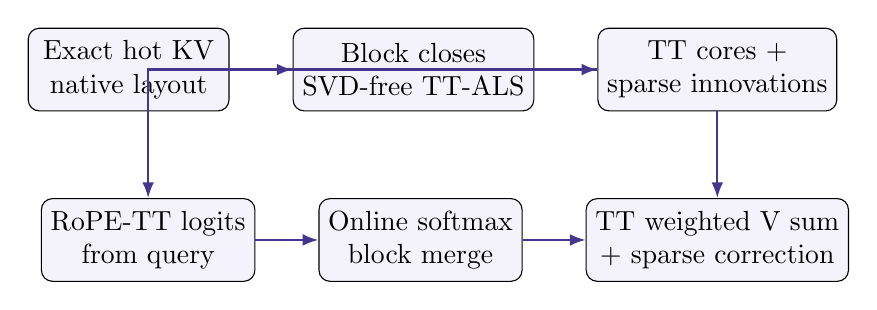
\begin{tikzpicture}[
  box/.style={draw,rounded corners,minimum height=1.05cm,minimum width=2.55cm,align=center,fill=soft},
  arr/.style={-{Latex[length=2mm]},thick,accent}]
\node[box] (hot) {Exact hot KV\\native layout};
\node[box,right=8mm of hot] (age) {Block closes\\SVD-free TT-ALS};
\node[box,right=8mm of age] (store) {TT cores +\\sparse innovations};
\node[box,below=11mm of store] (val) {TT weighted V sum\\+ sparse correction};
\node[box,left=8mm of val] (soft) {Online softmax\\block merge};
\node[box,left=8mm of soft] (key) {RoPE-TT logits\\from query};
\draw[arr] (hot)--(age); \draw[arr] (age)--(store);
\draw[arr] (store)--(val); \draw[arr] (store.west) -| (key.north);
\draw[arr] (key)--(soft); \draw[arr] (soft)--(val);
\end{tikzpicture}
\end{center}

\section{Theory targets}
\label{sec:theory}

The proposal separates elementary guarantees that can be completed early from ambitious results
that are contingent on the final algorithm.

\begin{targettheorem}[One-query attention-output error]
\leavevmode\par\noindent
Let $\epsilon_K=\max_s\norm{K_s-\widehat K_s}_2$,
$\epsilon_V=\max_s\norm{V_s-\widehat V_s}_2$, and
$V_{\max}=\max_s\norm{\widehat V_s}_2$. Then establish an explicit bound of the form
\[
\norm{o(q)-\widehat o(q)}_2
\le \epsilon_V + 2V_{\max}\frac{\norm q_2\epsilon_K}{\sqrt d},
\]
with a tighter version using retained sparse innovations and observed attention mass.
\end{targettheorem}

The proof decomposes the error into value approximation and probability-vector perturbation, uses
$\norm{s-\widehat s}_\infty\le\norm q_2\epsilon_K/\sqrt d$, and bounds the softmax Jacobian from
$\ell_\infty$ to $\ell_1$. RoPE does not enlarge the key norm because each rotation is orthogonal.

\begin{targettheorem}[Robust residual selection]
For a query set contained in the span-plus-radius model
$q=Q_ba+u$, $\norm u_2\le\rho$, show that the influence score upper-bounds the worst-case logit
error of each omitted token. Use this to derive a sufficient residual budget for a requested
$\ell_\infty$ logit tolerance.
\end{targettheorem}

\begin{proposition}[Payback admission]
Let $T_c$ be one-time block compression time and let $\Delta T=T_{\rm dense/read}-T_{\rm TT/query}$.
If $\Delta T>0$, compression improves cumulative time after
$N_{\rm pay}=\lceil T_c/\Delta T\rceil$ future queries. If $\Delta T\le0$, the runtime must reject
TT storage for that block.
\end{proposition}

No universal-compressibility theorem is claimed. Recent minimax analysis shows that accurate KV
compression requires assumptions on intrinsic cache structure~\cite{riskkv}; the paper will state
and empirically test those assumptions.

\section{System design and cost model}

For uniform internal rank $r$ and dyadic $B=2^p$, approximate per-head storage is
$2pr^2+rd$ scalars per K or V block. A prefix-reuse traversal targets $O(Br^2+rd)$ key work and
$O(Br^2+rd)$ value work, compared with $O(Bd)$ arithmetic and $O(Bd)$ reads for dense attention.
The TT path is plausible only when rank and kernel launch overhead are small enough that reduced
memory traffic dominates extra core contractions.

The controller profiles each $(\ell,h,B,r)$ configuration and stores a lookup table containing
physical bytes, compression time, and direct-kernel latency. At block close it predicts remaining
queries from the requested maximum generation length and chooses among native, INT4, and TT plus
sparse residual. This fallback is part of the correctness of the systems claim, not an ablation.

Implementation stages are:
\begin{enumerate}[leftmargin=1.55em,itemsep=2pt]
\item PyTorch reference for TT fitting, direct logits, direct value aggregation, and equality tests.
\item CUDA prototype with fixed $B\in\{128,256,512\}$ and ranks $r\in\{4,8,12,16\}$.
\item Fused online-softmax merge across hot, native/INT4, and TT blocks.
\item Hugging Face cache integration for LLaMA/Mistral/Qwen-style GQA and MHA.
\item Jetson Orin measurements plus one desktop/datacenter NVIDIA GPU to avoid device-specific claims.
\end{enumerate}

\section{Experimental plan}
\label{sec:experiments}

\subsection{Research questions}
\begin{enumerate}[leftmargin=1.55em,itemsep=2pt]
\item Do per-layer, per-head aged KV blocks have low causal TT ranks before and after RoPE?
\item Does attention-weighted fitting dominate Frobenius TT fitting at matched bytes?
\item Does analytic RoPE contraction reduce rank or latency relative to post-RoPE TT?
\item Do sparse innovations prevent routing failures under retrieval and reasoning workloads?
\item At what context, rank, and device does TT cross its payback point against BF16 and INT4?
\end{enumerate}

\subsection{Models, workloads, and baselines}
Start with LLaMA-3.2-1B/3B for development, then evaluate at least two architecture families and
both GQA and MHA where resources allow. Workloads include PG19 perplexity, RULER retrieval,
LongBench, GSM8K or an equivalent reasoning set, and controlled adversarial prompts with isolated
rare facts. Context lengths must include $4$K, $8$K, $16$K, and the longest length supported by the
device without extrapolation artifacts.

Baselines are full BF16/FP16, native INT8/INT4 KV, KIVI~\cite{kivi}, Palu, Eigen Attention,
OjaKV, RAP, DecoQuant, JoLT, and a reconstruction-based TT implementation. Quantization is a
mandatory baseline because evidence suggests it can dominate rank reduction at matched
budgets~\cite{quantdom}. If code for a July 2026 preprint is unavailable, reproduce its reported
setting or clearly label a result as paper-reported rather than locally reproduced.

\subsection{Metrics and ablations}
Report physical allocated bytes, bytes read per decoded token, fit latency, payback queries,
time-to-first-token, inter-token latency (median/P95), tokens/s, energy/token, maximum context before
OOM, perplexity, exact-match/task accuracy, and attention-output error. Every quality plot uses
matched physical bytes; every speed plot includes compression cost.

Required ablations: TT versus TT-SVD (offline quality only); ALS sweep count; token radix/order;
pre- versus post-RoPE; query-weighted versus Frobenius objective; residual type and budget; direct
versus reconstructed attention; rank controller; factor quantization; and native/INT4 fallback.

\section{Reviewer attacks and pre-registered failure cases}

\begin{riskbox}
Stop or pivot if, on two model families, (i) median useful TT rank exceeds the direct-kernel
break-even rank, (ii) compression payback exceeds 25\% of expected remaining generation, or
(iii) INT4 matches quality while remaining faster and no larger. A tensor preference is not a
reason to continue a dominated method.
\end{riskbox}

Likely reviewer attacks and defenses:
\begin{itemize}[leftmargin=1.5em,itemsep=2pt]
\item \textbf{``TT is only a different factorization.''} Defense: isolate the value of causal update,
RoPE operator, direct kernel, and attention-aware residual; do not claim factorization novelty.
\item \textbf{``The method is slower than quantization.''} Defense: matched-byte kernel results and
payback admission; report rejection frequency rather than hiding unfavorable layers.
\item \textbf{``Future queries are unknown.''} Defense: robust span-plus-radius bound, multi-query
evaluation, and distribution-shift tests.
\item \textbf{``Tensor ranks are layout artifacts.''} Defense: pre-register radix/mode-order search
and test ranks across domains and random permutations.
\item \textbf{``One Jetson is not a top-venue evaluation.''} Defense: Jetson demonstrates the target
constraint; a second NVIDIA platform establishes portability and separates method from device.
\end{itemize}

\section{Paper outline and contribution discipline}

\begin{enumerate}[leftmargin=1.55em,itemsep=3pt]
\item \textbf{Introduction:} memory traffic, why storage-only compression is insufficient, and the
single key idea.
\item \textbf{Background/diagnosis:} TT, RoPE, strongest cache baselines, and measured naive-TT
failure.
\item \textbf{CATT-KV representation:} causal tensorization and SVD-free age-triggered fitting.
\item \textbf{Direct attention:} RoPE operator, logits traversal, V aggregation, sparse merge.
\item \textbf{Controller and analysis:} attention objective, error bound, memory/operation counts,
payback admission.
\item \textbf{Evaluation:} quality, physical memory, latency, energy, ablations, failure regions.
\item \textbf{Limitations:} rank explosion, short-context overhead, architecture dependence, and
custom-kernel maintenance.
\end{enumerate}

The paper should claim three technical contributions and one evaluation contribution at most. It
must not simultaneously claim a new benchmark, universal theory, and a new serving system.

\section{Execution schedule}

\begin{center}
\small
\renewcommand{\arraystretch}{1.2}
\begin{tabularx}{\textwidth}{@{}p{1.6cm}p{3.0cm}X@{}}
\toprule
\textbf{Weeks} & \textbf{Deliverable} & \textbf{Exit criterion} \\
\midrule
1--2 & Recorded-KV structural pilot & TT rank/byte curves and direct-contraction microbenchmark \\
3--5 & Reference method & SVD-free fit, sparse residual, numerical equivalence tests \\
6--9 & CUDA direct kernels & No dense allocation; positive break-even region demonstrated \\
10--12 & Model integration & Stable generation, full-cache parity at uncompressed rank \\
13--16 & Evaluation & Two model families, all required baselines and ablations \\
17--20 & Theory and writing & Verified bounds, artifact, complete paper draft \\
\bottomrule
\end{tabularx}
\end{center}

\section{Final verdict}

\begin{claimbox}
If the gates pass, the defensible thesis is: \emph{causal Tensor-Train compression can move old-KV
attention from dense memory streaming to bounded-rank core contraction, while RoPE-aware sparse
innovations preserve routing and a payback controller prevents negative-speedup cases.}
\end{claimbox}

The idea is an \textbf{accept-with-major-revisions research direction}: its logic chain is strong,
but novelty and feasibility depend on the direct kernel beating INT4 in a meaningful region. The
appropriate venue is NeurIPS/ICLR if the attention objective and guarantees lead; MLSys or ACM
ASPLOS if kernel, memory traffic, and end-to-end payback lead; ACM MobiSys if energy/thermal edge
deployment becomes the principal result.

\begin{thebibliography}{99}\small

\bibitem{decoquant} P. Liu et al. \emph{Unlocking Data-free Low-bit Quantization with Matrix
Decomposition for KV Cache Compression.} ACL 2024. \url{https://aclanthology.org/2024.acl-long.133/}

\bibitem{jolt} R. Krishnan and V. Schulz. \emph{A JoLT for the KV Cache: Near-Lossless KV Cache
Compression via Joint Tucker and JL-Residual Allocation for LLMs.} arXiv:2607.12550, 2026.
\url{https://arxiv.org/abs/2607.12550}

\bibitem{tuckerkv} H.-M. Hsu. \emph{Tucker-KV: Provable Tucker Compression of KV Caches with
Monotone Refinement and Near-Optimal Budgeting.} OpenReview, 2025--2026.
\url{https://openreview.net/forum?id=aQ6RiOijal}

\bibitem{palu} C.-C. Chang et al. \emph{Palu: KV-Cache Compression with Low-Rank Projection.}
ICLR 2025. \url{https://openreview.net/forum?id=LWMS4pk2vK}

\bibitem{eigen} U. Saxena et al. \emph{Eigen Attention: Attention in Low-Rank Space for KV Cache
Compression.} Findings of EMNLP 2024. \url{https://aclanthology.org/2024.findings-emnlp.899/}

\bibitem{ojakv} Y. Zhu et al. \emph{OjaKV: Context-Aware Online Low-Rank KV Cache Compression.}
Findings of ACL 2026. \url{https://aclanthology.org/2026.findings-acl.494/}

\bibitem{rap} J. Xin et al. \emph{RAP: KV-Cache Compression via RoPE-Aligned Pruning.}
arXiv:2602.02599, 2026. \url{https://arxiv.org/abs/2602.02599}

\bibitem{onlinett} H. Takeda, Y. Miyatake, and D. Furihata. \emph{Online TT-ALS for Streaming
Tensor Decomposition with Incremental Orthogonalization.} arXiv:2606.31061, 2026.
\url{https://arxiv.org/abs/2606.31061}

\bibitem{stta} D. Kressner, B. Vandereycken, and R. Voorhaar. \emph{Streaming Tensor Train
Approximation.} SIAM J. Scientific Computing, 2023. \url{https://arxiv.org/abs/2208.02600}

\bibitem{riskkv} L. Haverbeck et al. \emph{The Risk of KV Cache Compression.}
arXiv:2607.01520, 2026. \url{https://arxiv.org/abs/2607.01520}

\bibitem{quantdom} S. Salfati. \emph{Quantization Dominates Rank Reduction for KV-Cache
Compression.} arXiv:2604.11501, 2026. \url{https://arxiv.org/abs/2604.11501}

\bibitem{kivi} Z. Liu et al. \emph{KIVI: A Tuning-Free Asymmetric 2bit Quantization for KV Cache.}
ICML 2024. \url{https://arxiv.org/abs/2402.02750}

\end{thebibliography}

\end{document}
